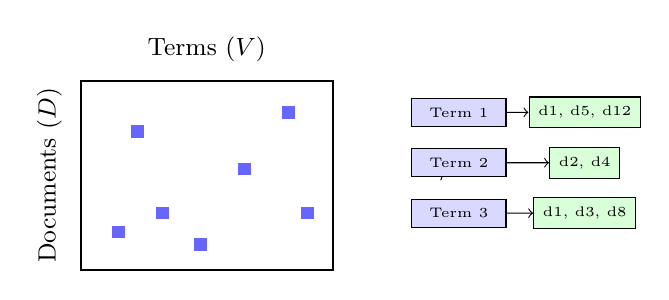
\begin{tikzpicture}[scale=0.8]
    % Matrix outline
    \draw[thick] (0,0) rectangle (4,3);
    \node[rotate=90] at (-0.5, 1.5) {\small Documents ($D$)};
    \node at (2, 3.5) {\small Terms ($V$)};
    
    % Sparse points
    \foreach \x/\y in {0.5/0.5, 1.2/0.8, 0.8/2.1, 2.5/1.5, 3.2/2.4, 1.8/0.3, 3.5/0.8} {
        \fill[blue!60] (\x, \y) rectangle (\x+0.2, \y+0.2);
    }
    
    \node[right=4.2cm] at (0, 1.5) {$\rightarrow$};
    
    % Index structure
    \begin{scope}[shift={(6,0.5)}]
        \node[draw, fill=blue!15, minimum width=1.2cm] (t1) at (0, 2) {\tiny Term 1};
        \node[draw, fill=blue!15, minimum width=1.2cm] (t2) at (0, 1.2) {\tiny Term 2};
        \node[draw, fill=blue!15, minimum width=1.2cm] (t3) at (0, 0.4) {\tiny Term 3};
        
        \node[draw, fill=green!15] (p1) at (2, 2) {\tiny d1, d5, d12};
        \node[draw, fill=green!15] (p2) at (2, 1.2) {\tiny d2, d4};
        \node[draw, fill=green!15] (p3) at (2, 0.4) {\tiny d1, d3, d8};
        
        \draw[->] (t1) -- (p1);
        \draw[->] (t2) -- (p2);
        \draw[->] (t3) -- (p3);
    \end{scope}
\end{tikzpicture}
